        \documentclass{standalone}
        \usepackage{tikz}
        \usepackage{amsmath}
        \begin{document}
        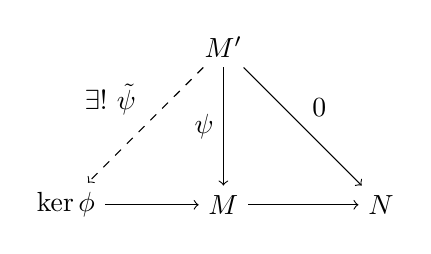
\begin{tikzpicture}

    \node (T) at (0,0) {$M^\prime$};
    \node (M) at (0,-2) {$M$};
    \node (N) at (2,-2) {$N$};
    \node (ker) at (-2,-2) {$\ker \phi$};
    \draw[->] (T) -- node[left] {$\psi$} (M);
    \draw[->] (T) -- node[above right] {$0$} (N);
    \draw[->,dashed] (T) -- node[above left] {$\exists ! ~\tilde{\psi}$} (ker);
    \draw[->] (ker) -- (M);
    \draw[->] (M) -- (N);
        \end{tikzpicture}
        \end{document}
